\documentclass[aspectratio=169]{beamer}

\usepackage{mystyle}

\title{Measuring the Information Content of VIX Volatility}
\author{Context: Humboldt Project\\
Supervisor: Prof. Franziska Peter\\
Author: Sophia Gläser (7. Semester BA CME)}
\date{\small \today}

\addbibresource{./bib/bibliography.bib} 

\begin{document}

\begin{frame}
\maketitle
\end{frame}

\begin{frame}
\frametitle{Table of Contents}
\tableofcontents
\end{frame}

\section{Introduction}

\begin{frame}
\frametitle{Motivation: Why this project? Why does Volatility matter?}
	\begin{itemize}
	\item For the stability of the financial system, precise risk measurement is of great importance
	\begin{itemize}
	\item Volatility is closely related to risk 
	\item it is crucial input to risk measures, such as the Value at Risk\footnote{The Value at Risk is a quantile of the loss function, used for example by banks to estimate the amount of assets needed to cover possible losses. It estimates which loss is not going to be exceeded in a given time interval, for a given probability}
	\end{itemize}
	\item Moreover volatility is used for..
	\begin{itemize}
	\item .. the pricing of financial instruments, such as derivatives
	\item .. the risk-return trade-off and therefore management decisions
	\end{itemize}
	\end{itemize}
\end{frame}

\begin{frame}
\frametitle{More closely: What exactly is Volatility?}
	\begin{itemize}
	\item In Finance, we are usually interested in the \textit{conditional} standard deviation from the expected value of the underlying asset return \parencite{tsay2005}
	\item What causes asset price movement and thus volatility?
	\begin{itemize}
	\item Assuming Market efficiency (as introduced by \citeauthor{fama1970}), stock prices incorporate all available information from the market, because of competition and free entry 
	\item But that does not does not give us information about the distribution of stock prices
	\end{itemize}
	\end{itemize}
\end{frame}

\begin{frame}
\frametitle{The Problem: Why is it so hard to measure and forecast volatility?}
	\begin{itemize}
	\item Volatility is not directly observable
	\begin{itemize}
	\item We can estimate it for a given time period 
	\item However, stock volatility consists of intraday and overnight volatility, each containing different information
	\end{itemize}
	%
	\item But we observe some characteristics about volatility, and can thus use econometric models, that best ``copy'' these stylized facts
	\begin{itemize}
	\item ..
	\end{itemize}
	%
	\end{itemize}
\end{frame}

\begin{frame}
\frametitle{Maybe a solution: How volatility has been calculated so far}
	\begin{itemize}
	\item According to the observed characteristics (and making some assumptions), we can use (econmetric) models to estimate volatility
	\begin{itemize}
	\item Econometric models using historic volatility (e.g. ARCH)
	\item Black-and-Scholes implied volatility
	\item ...
	\end{itemize}
	\item So far Black-and Scholes implied volatility has proven to contain significant information for realized volatility
	\end{itemize}
\end{frame}

\begin{frame}
\frametitle{Black-and-Scholes implied volatility}
	\begin{itemize}
	\item Intuition behind Black-and-Scholes (BS) implied volatility
	\begin{itemize}
	\item The BS model is a model, that uses volatility to price options
	\item By using option prices from the market, it is possible to turn the calculation around and derive an \textit{option implied volatility}
	\end{itemize}
	%
	\item there are however some problems with the BS implied volatility
	\begin{itemize}
	\item The Black-and-Scholes model is mainly based on at-the-money options (fails to incorporate information contained in others)
	\item Most imprtantly The Black-and-Scholes model makes pricing assumptions (e.g. that stock prices follow geometric Brownian motion)
	\end{itemize}
	%
	\item $\rightarrow$ Joint hypothesis problem
	\begin{itemize}
	\item Testing for BS implied volatility is always a test of \textit{both} market efficiency and the BS pricing assumptions
	\item So far market efficiency per se is not testable
	\end{itemize}
	\end{itemize}
\end{frame}

\begin{frame}
\frametitle{Solving the joint hypothesis problem: Model-free implied volatility}
	\begin{itemize}
	\item to correct for the model specification problems with the BS implied volatility 
	\item one of the fist model-free implied volatility indices was the VIX from CBOE
	\item the VIX uses options 
	\end{itemize}
\end{frame}

\section{Data}

\begin{frame}
\frametitle{Volatility of S\&P 500}
	\begin{figure}
	\centering
	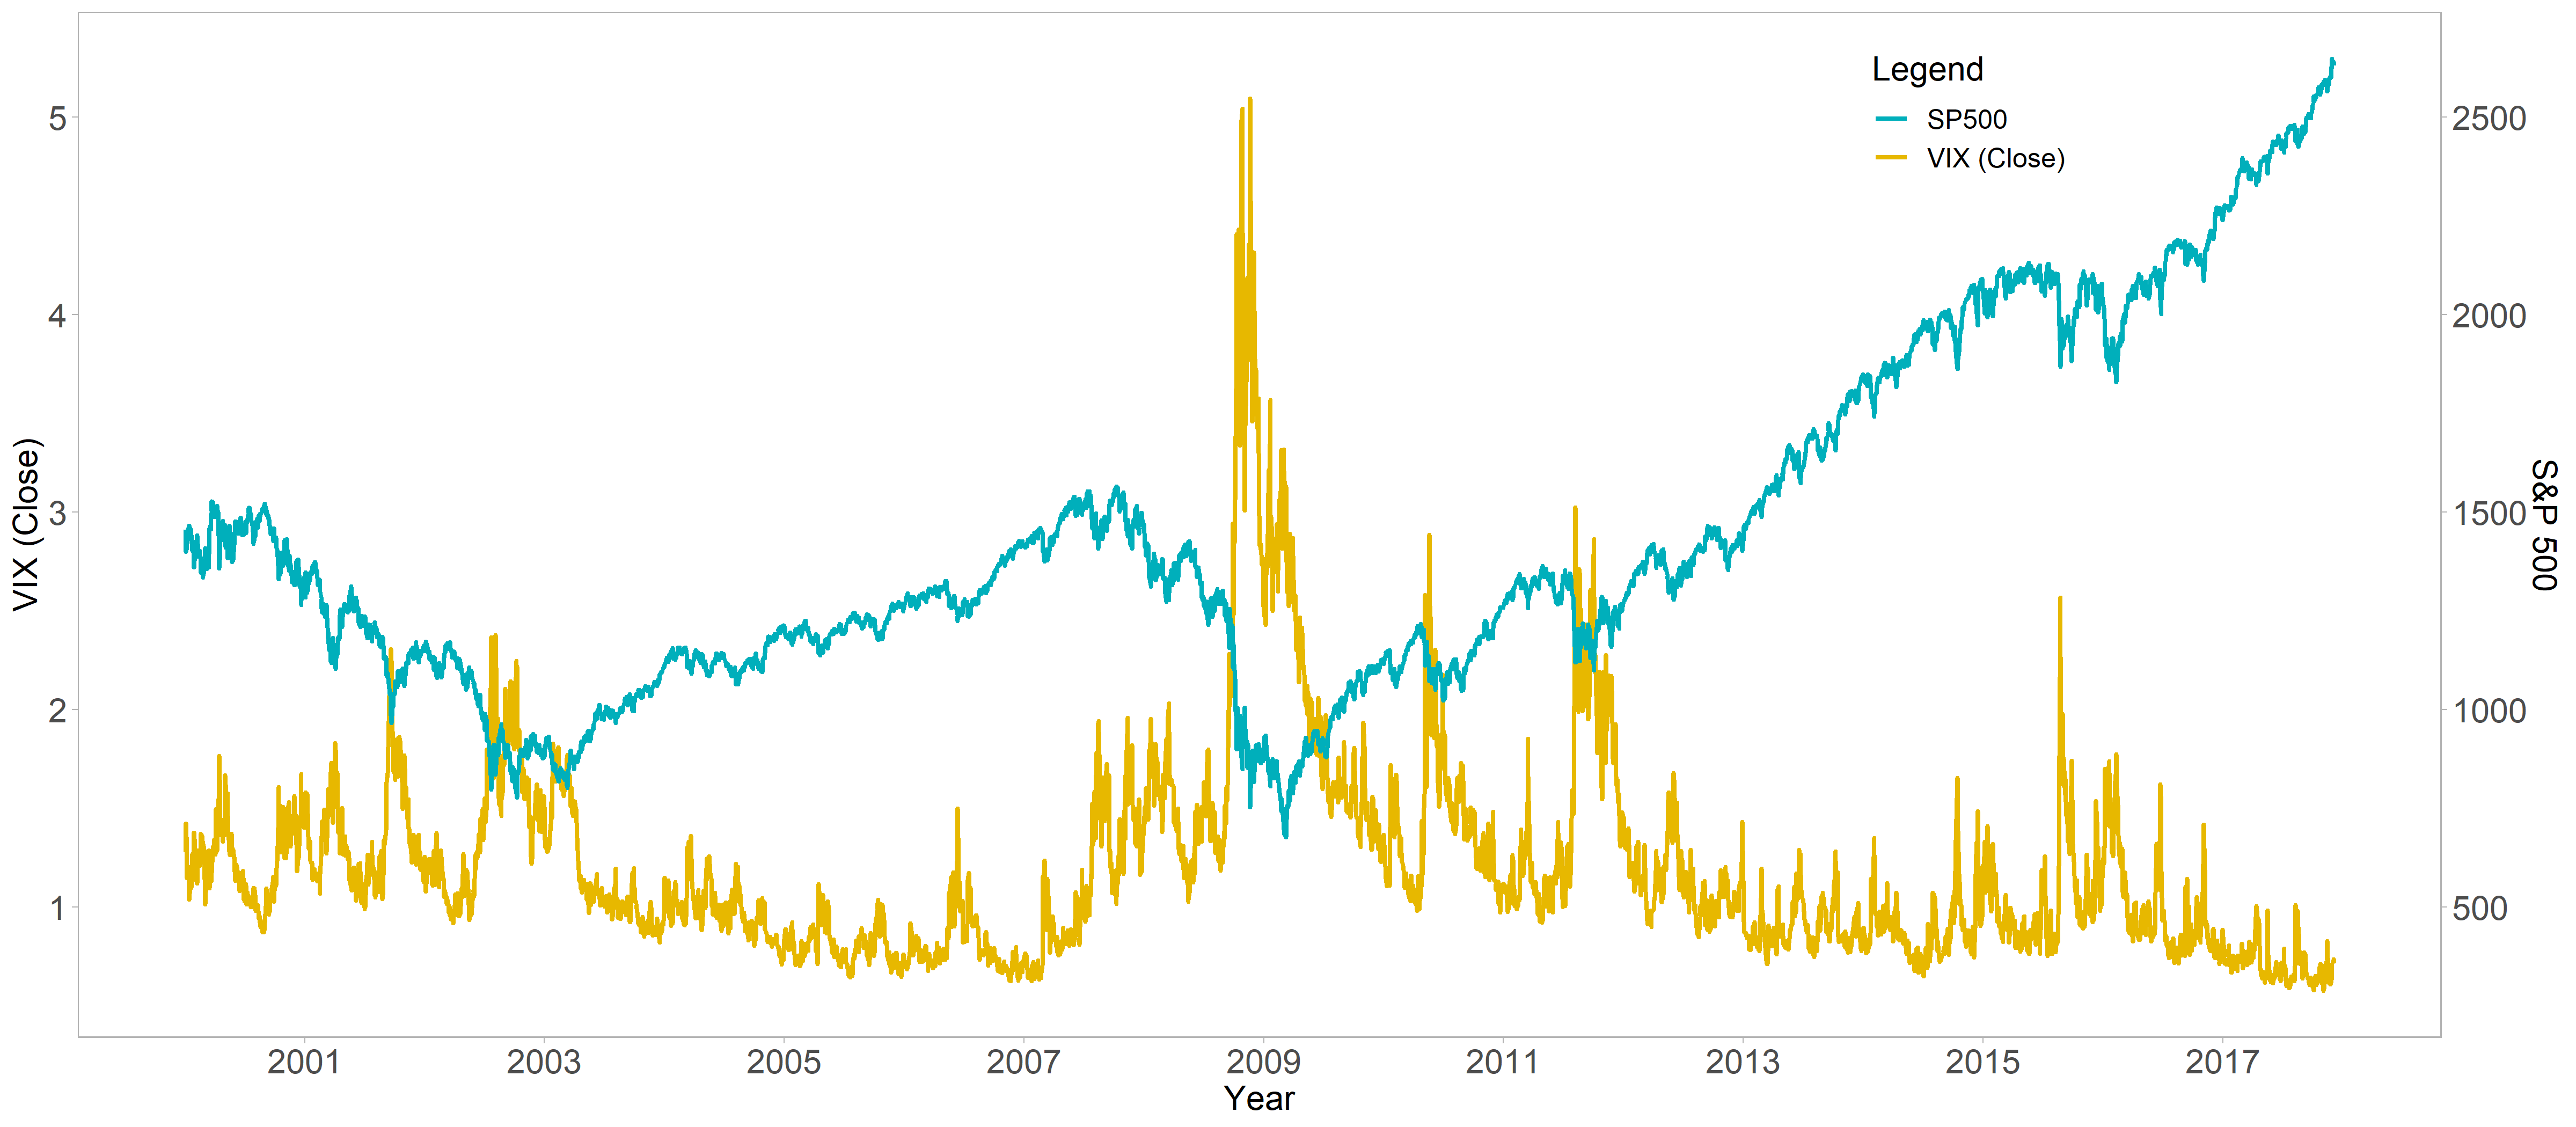
\includegraphics[scale = 0.35]{graphics/SPandViX.png}
	\end{figure}
\end{frame}


\section{Method}

\begin{frame}
\frametitle{}
	\begin{itemize}
	\item Regression of realized volatility on historic volatility
	\end{itemize}
\end{frame}


\section{Results so far}

\begin{frame}
\frametitle{}
	\begin{itemize}
	\item
	\end{itemize}
\end{frame}


\section{Possible Problems coming up}

\begin{frame}
\frametitle{Questions currently to solve}
	\begin{itemize}
	\item Having gathered all this information about volatility measurement, what is the most accurate way to set up my regression?
	
	\end{itemize}
\end{frame}

\section*{Sources}
\begin{frame}
\printbibliography
\end{frame}

\section{Appendix}
\begin{frame}
\frametitle{The Black and Scholes Equation}
%
\begin{minipage}{0.6\textwidth}
\begin{small}
%
price of an option over time:
\begin{equation}
	\frac{\partial \mathrm C}{ \partial \mathrm t } + \frac{1}{2}\sigma^{2} \mathrm S^{2} \frac{\partial^{2} \mathrm C}{\partial \mathrm C^2}
	+ \mathrm r \mathrm S \frac{\partial \mathrm C}{\partial \mathrm S}\ =
	\mathrm r \mathrm C 
	\label{eq:1}
\end{equation}
%
calculate the price of European call and put option: 
\begin{equation}
	\mathrm C(\mathrm S,\mathrm t)= \mathrm N(\mathrm d_1)\mathrm S - \mathrm N(\mathrm d_2) \mathrm K \mathrm e^{-rt}
	\label{eq:2}
\end{equation}
\vspace{-3pt}
%
\begin{equation}
	\mathrm d_1= \frac{1}{\sigma \sqrt{\mathrm t}} \left[\ln{\left(\frac{S}{K}\right)} + t\left(r + \frac{\sigma^2}{2} \right) \right]
\end{equation}
\vspace{-3pt}
%
\begin{equation}
	\mathrm d_2= \frac{1}{\sigma \sqrt{\mathrm t}} \left[\ln{\left(\frac{S}{K}\right)} + t\left(r - \frac{\sigma^2}{2} \right) \right]
\end{equation}
\vspace{-3pt}
%
\begin{equation}
	N(x)=\frac{1}{\sqrt{2\pi}} \int_{-\infty}^{x} \mathrm e^{-\frac{1}{2}z^2} dz
	\label{eq:5}
\end{equation}
\end{small}
\end{minipage}
%
\begin{minipage}{0.35\textwidth}
\begin{footnotesize}
\begin{itemize}
	\item[] C = Call option price 
	\item[] S = Current stock price
	\item[] K = Strike price of the option
	\item[] r = risk-free interest rate (a number between 0 and 1)
	\item[] $\sigma$ = volatility of the stocks return (a number between 0 and 1)
	\item[] t = time to option maturity (in years)
	\item[] N = normal cumulative distribution function
\end{itemize}
\end{footnotesize}
\end{minipage}
%
\end{frame}

\begin{frame}
\frametitle{The VIX Equation}
\end{frame}



\end{document}
